\documentclass[10pt, compress, aspectratio=169]{beamer}

% DZ: My MikTeX freezes when trying to compile the source with the metropolis theme.
%\usetheme{metropolis}
\usepackage{appendixnumberbeamer}

\usepackage{tikz-dependency}
\usepackage{caption}
\usepackage{booktabs}
\usepackage{url}
\usepackage{fontspec}
\usepackage[scale=2]{ccicons}

\usepackage{pgfplots}
\usepgfplotslibrary{dateplot}

\usepackage{xspace}
\newcommand{\themename}{\textbf{\textsc{metropolis}}\xspace}

% commands from the paper
\newcommand{\udtag}[1]{{\ll \textsc{#1}}}
\newcommand{\udlabel}[1]{{\tt #1}}
\newcommand{\tgl}[1]{{\em #1}}
% commands from the paper
\newfontfamily\cyr[Scale=0.8,Script=Cyrillic]{DejaVu Sans}
% Dan's stuff.
\usepackage{comment}
\newcommand{\todo}[1]{\textcolor{red}{[TODO: {#1}]}} % komentáře TODO

\newcommand{\myleftarrow}[1][45]{%
  \mathrel{%
    \text{$
     \begin{tikzpicture}[baseline = -0.5ex]
       \node[inner sep=0pt,outer sep=0pt,rotate = #1] (a) at (0,0)  {$\xleftarrow{}$};
    \end{tikzpicture}
    $}%
  }%
}%

\newcommand{\myrightarrow}[1][-45]{%
  \mathrel{%
    \text{$
     \begin{tikzpicture}[baseline = -0.5ex]
       \node[inner sep=0pt,outer sep=0pt,rotate = #1] (a) at (0,0)  {$\xrightarrow{}$};
    \end{tikzpicture}
    $}%
  }%
}%

\setbeamertemplate{navigation symbols}{}
\setbeamertemplate{footline}{
  \hfill%
  \usebeamercolor[fg]{page number in head/foot}%
  \usebeamerfont{page number in head/foot}%
  \setbeamertemplate{page number in head/foot}[framenumber]%
  \usebeamertemplate*{page number in head/foot}\kern3.5em\vskip10pt%
}
\newcommand{\nologo}{\setbeamertemplate{logo}{}}



\title{Tutorial on Universal Dependencies\\
{\small Adding a new language to UD}}
\date{\today}
\date{}
\author{%
Marie-Catherine de Marneffe\inst{1}
\and
Joakim Nivre\inst{2}
\and
\textbf{Daniel Zeman}\inst{3}
\vspace{0.5cm}
}
\institute[shortinst]{%
\inst{1}
FNRS,
Université catholique de Louvain, Belgium
\and
\inst{2}
Department of Linguistics and Philology,
Uppsala University, Sweden
\and
\inst{3}
Institute of Formal and Applied Linguistics,
Charles University, Prague, Czechia
}
\logo{\hfill
\includegraphics[height=1.25cm]{images/ud-logo-transp.png}}


\begin{document}

\maketitle

\begin{frame}
  \frametitle{Two Scenarios}
  \begin{center}
  \begin{tabular}{cc}
    \hline
            ~ & ~ \\
    \multicolumn{2}{c}{{\large You want your language in UD}} \\
            ~ & ~ \\
      $\myleftarrow$  & $\myrightarrow$ \\
            ~ & ~ \\
    Existing treebank & No existing treebank  \\
    You have permission & No permission/licence \\
            ~ & ~ \\
         $\downarrow$ & $\downarrow$ \\
            ~ & ~ \\
    \textbf{Treebank conversion} & \textbf{Building from scratch} \\
            ~ & ~ \\
    \hline
  \end{tabular}
  \end{center}
\end{frame}


\begin{frame}
  \frametitle{Common Steps}
  \begin{columns}
    \column{0.7\textwidth}
    \textbf{First steps}
    \begin{itemize}
      \item Get an account in GitHub
      \begin{itemize}
        \item All development goes on here
      \end{itemize}
    \end{itemize}
    \textbf{Get in contact}
    \begin{itemize}
      \item Ask the release team (= Dan) to set up a repository
      \item Get in contact with any other teams working
        on your language, or a related one
      \item \alert{Register for the mailing list *}
    \end{itemize}
    \bigskip
    \begin{itemize}
      \item All contributors given broad edit rights to all data, docs, and
          tools repositories
      \item Fully trust-based setup, {\tt git} giving a safety net
    \end{itemize}
    \column{0.3\textwidth}
    \begin{center}
      \textbf{Release team}
      ~\\
      ~\\
      
\includegraphics[width=0.5\textwidth]{images/dan.png}
    \end{center}
  \end{columns}
  \bigskip
  {\small * \url{https://lists.uu.se/sympa/info/lingfil-ud}}
\end{frame}


\begin{frame}{Data}
  \begin{itemize}
    \item A GitHub repository for every treebank
      \begin{itemize}
        \item UD\_\{Language\}-\{Treebank\}
        \item \textbf{master} branch holds the most recent official
            release
        \item \textbf{dev} branch holds development data, not guaranteed
            to be valid
        \item Prescribed file names in the repository (extra files under
            \texttt{not-to-release})
        \item Recommended: push data to \texttt{dev} early, watch  the
            on-line validation page for errors
      \end{itemize}
    \item {\bf Official release:} LINDAT, May \& November, all treebanks
        which contain valid data
      \begin{itemize}
        \item \textbf{Data-freeze} period two weeks before the release
      \end{itemize}
    \item \textbf{Release checklist:}
        \url{https://universaldependencies.org/release_checklist.html}
  \end{itemize}
\end{frame}


{\nologo\begin{frame}{Validation}
  \begin{columns}[T] % align columns
    \begin{column}{.6\textwidth}
      \begin{itemize}
        \item Script(s) to validate treebank data
        \item Passing is compulsory
          \begin{itemize}
            \item Format validation
            \item Content (guidelines) validation
            \item Language-specific documentation
            \item File names and README contents
          \end{itemize}
        \item Runs automatically every time a treebank is updated
      \end{itemize}
    \end{column}
    \begin{column}{.4\textwidth}
      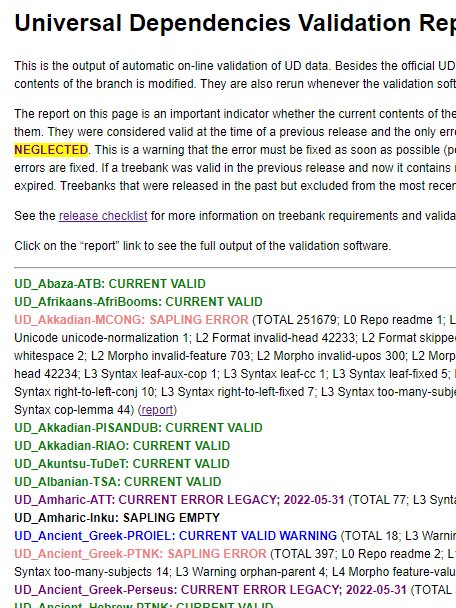
\includegraphics[width=\textwidth]{images/validation.png}
    \end{column}
  \end{columns}
  \url{https://quest.ms.mff.cuni.cz/udvalidator/}
\end{frame}}


\begin{frame}{Documentation}
  \begin{itemize}
    \item GitHub \emph{docs} repository, MarkDown pages $\rightarrow$ HTML
      \begin{itemize}
        \item Easy to add examples with tree visualizations
        \item Automatically regenerated on every push and published on
            \url{https://universaldependencies.org} (takes a few minutes)
      \end{itemize}
    \item One set of guidelines \textbf{per language} (not treebank)
      \begin{itemize}
        \item \alert{Mandatory} index page summarizing the language
          \begin{itemize}
            \item Template pre-generated when adding a new language
            \item Document as you annotate (or as you write conversion
                rules)
          \end{itemize}
        \item \alert{Mandatory} pages for lang-spec features and
            relations
        \item Optional other pages for features, relations and
            constructions
        \item Automatically generated treebank pages with statistics
      \end{itemize}
    \item
        \url{https://universaldependencies.org/contributing_language_specific.html}
    \item \url{http://spyysalo.github.io/annodoc/}
  \end{itemize}
\end{frame}


\begin{frame}{Language-specific Documentation}
  \begin{center}
    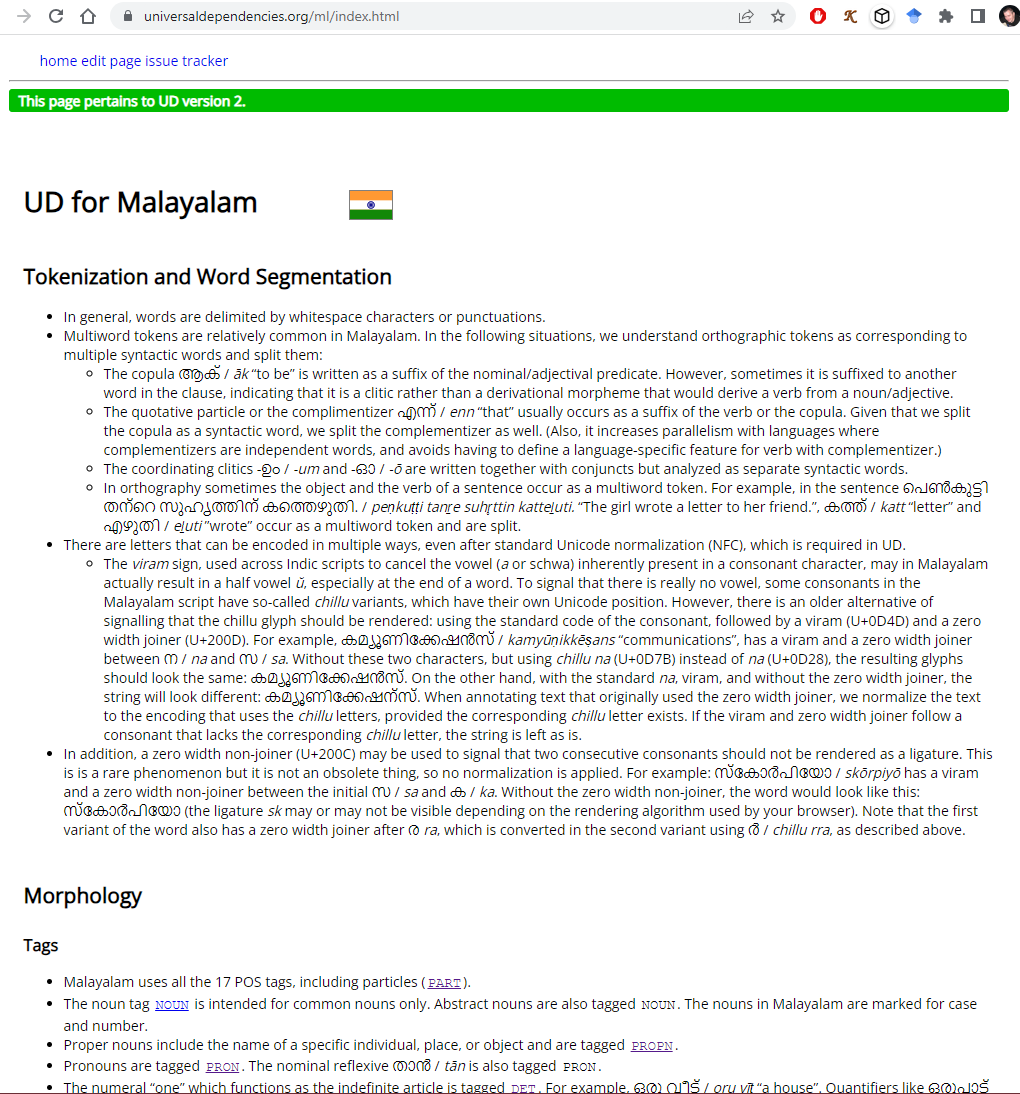
\includegraphics[width=0.95\textwidth]{images/docs-ml-index.png}
  \end{center}
\end{frame}


\begin{frame}{Language-specific Feature Documentation}
  \begin{center}
    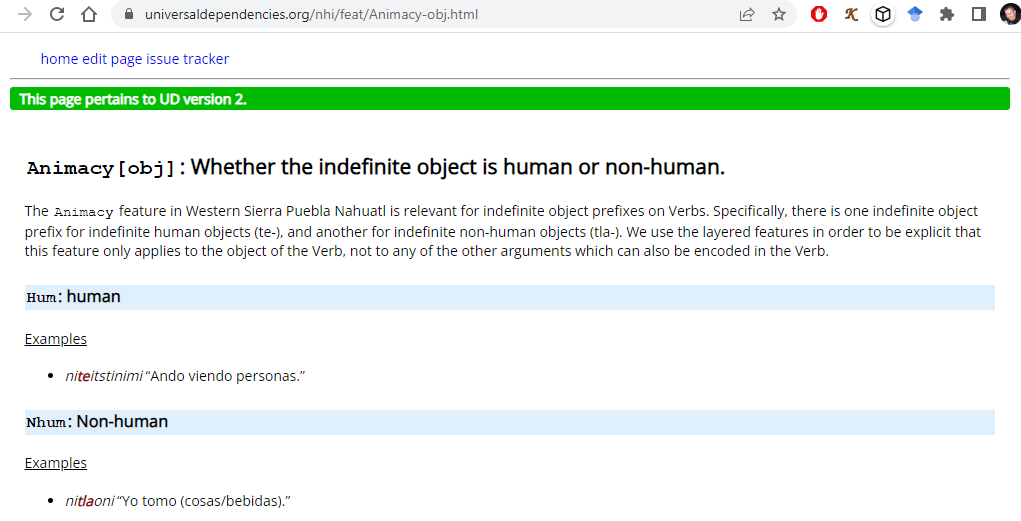
\includegraphics[width=0.95\textwidth]{images/docs-nhi-animacy-obj.png}
  \end{center}
\end{frame}


\begin{frame}{Language-specific Relation Documentation}
  \begin{center}
    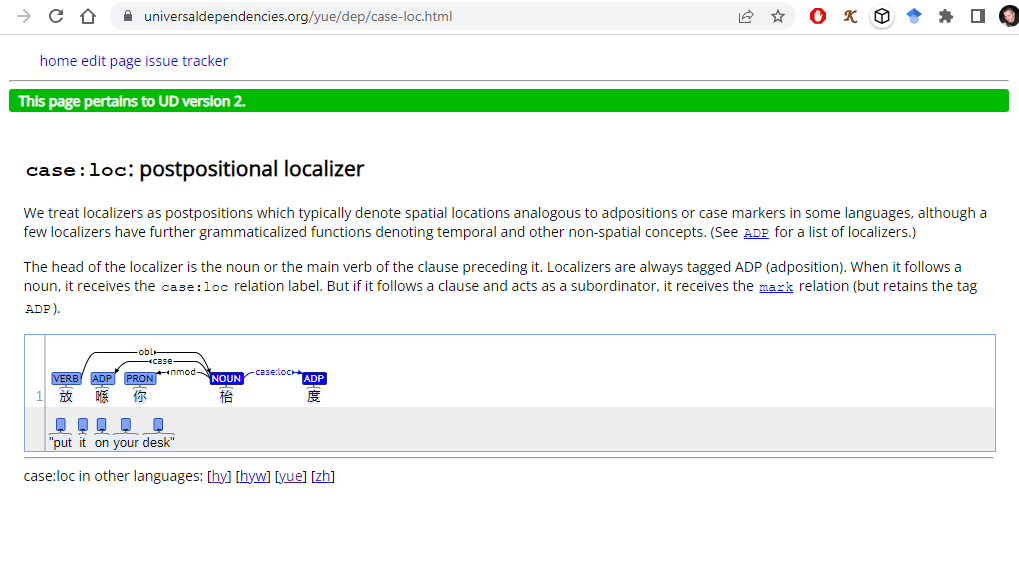
\includegraphics[width=0.95\textwidth]{images/docs-yue-case-loc.png}
  \end{center}
\end{frame}


\begin{frame}{Language-specific Rules for Validator}
  \begin{center}
    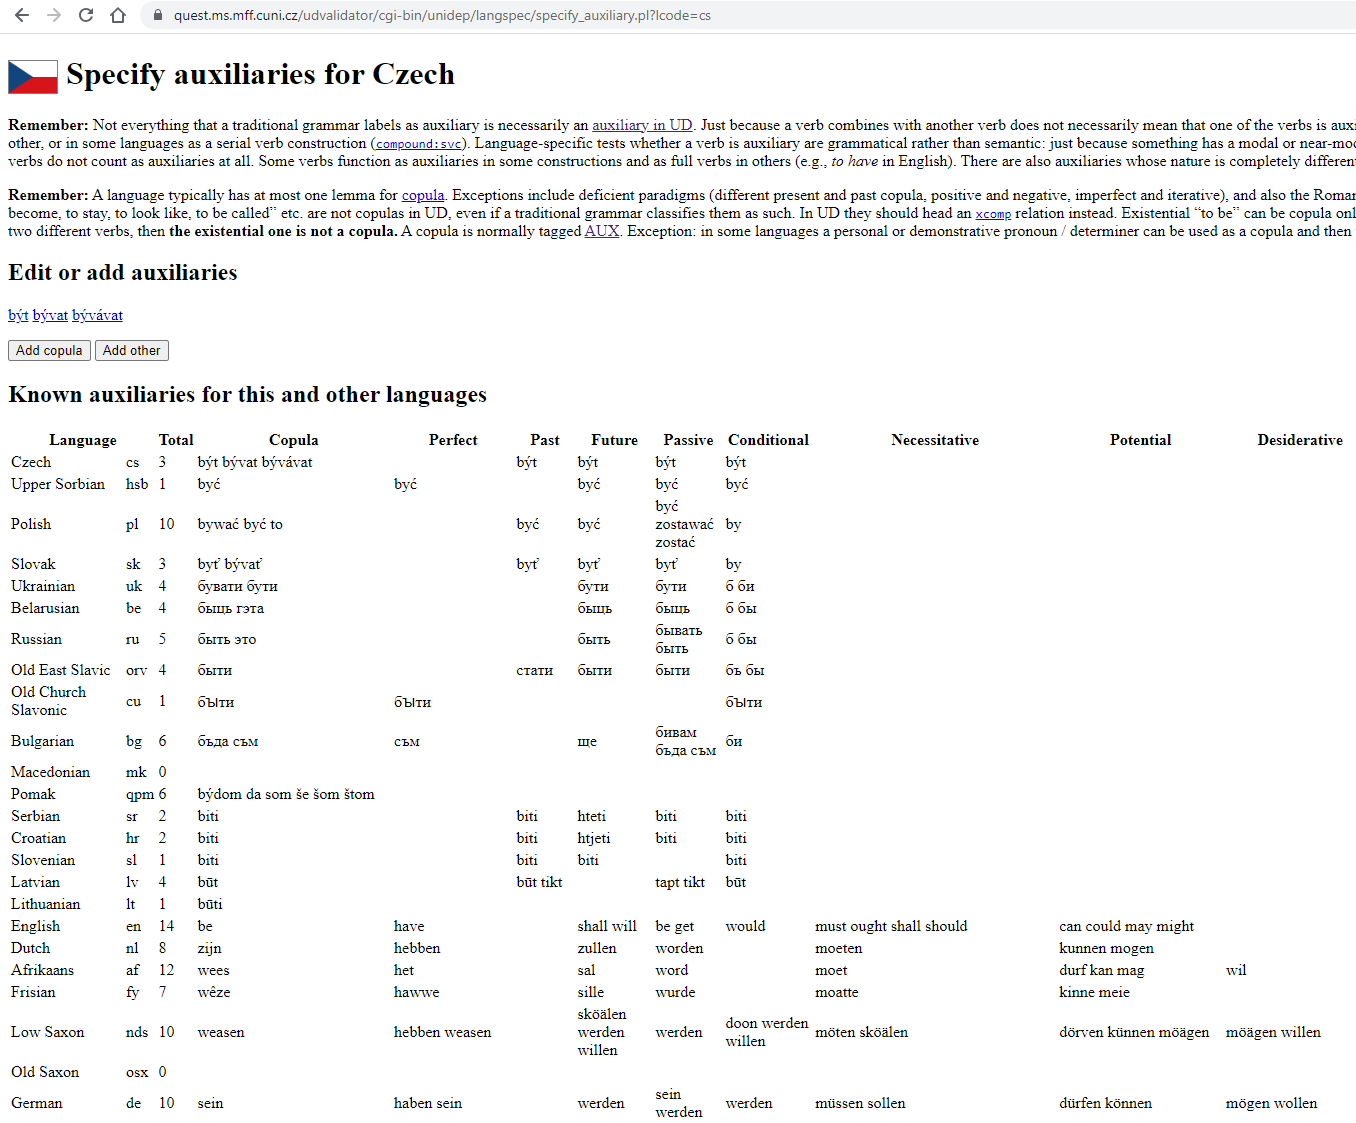
\includegraphics[width=0.95\textwidth]{images/validator-specify-auxiliaries-cs.png}
  \end{center}
\end{frame}


\begin{frame}{Language-specific Rules for Validator}
  \begin{itemize}
    \item \textbf{Morphological features}
      \begin{itemize}
        \item
            \url{https://quest.ms.mff.cuni.cz/udvalidator/cgi-bin/unidep/langspec/specify_feature.pl?lcode=}\alert{\url{cs}}
      \end{itemize}
    \bigskip
    \item \textbf{Dependency relations}
      \begin{itemize}
        \item
            \url{https://quest.ms.mff.cuni.cz/udvalidator/cgi-bin/unidep/langspec/specify_deprel.pl?lcode=}\alert{\url{cs}}
      \end{itemize}
    \bigskip
    \item \textbf{Auxiliaries and copulas}
      \begin{itemize}
        \item
            \url{https://quest.ms.mff.cuni.cz/udvalidator/cgi-bin/unidep/langspec/specify_auxiliary.pl?lcode=}\alert{\url{cs}}
      \end{itemize}
    \bigskip
    \item \alert{Do not make other people's treebanks invalid!}
  \end{itemize}
\end{frame}


\begin{frame}
  \frametitle{Linguistic Discussion}
  \begin{center}
    Linguistic discussion goes on under the \emph{docs} repository \\
    ~\\
    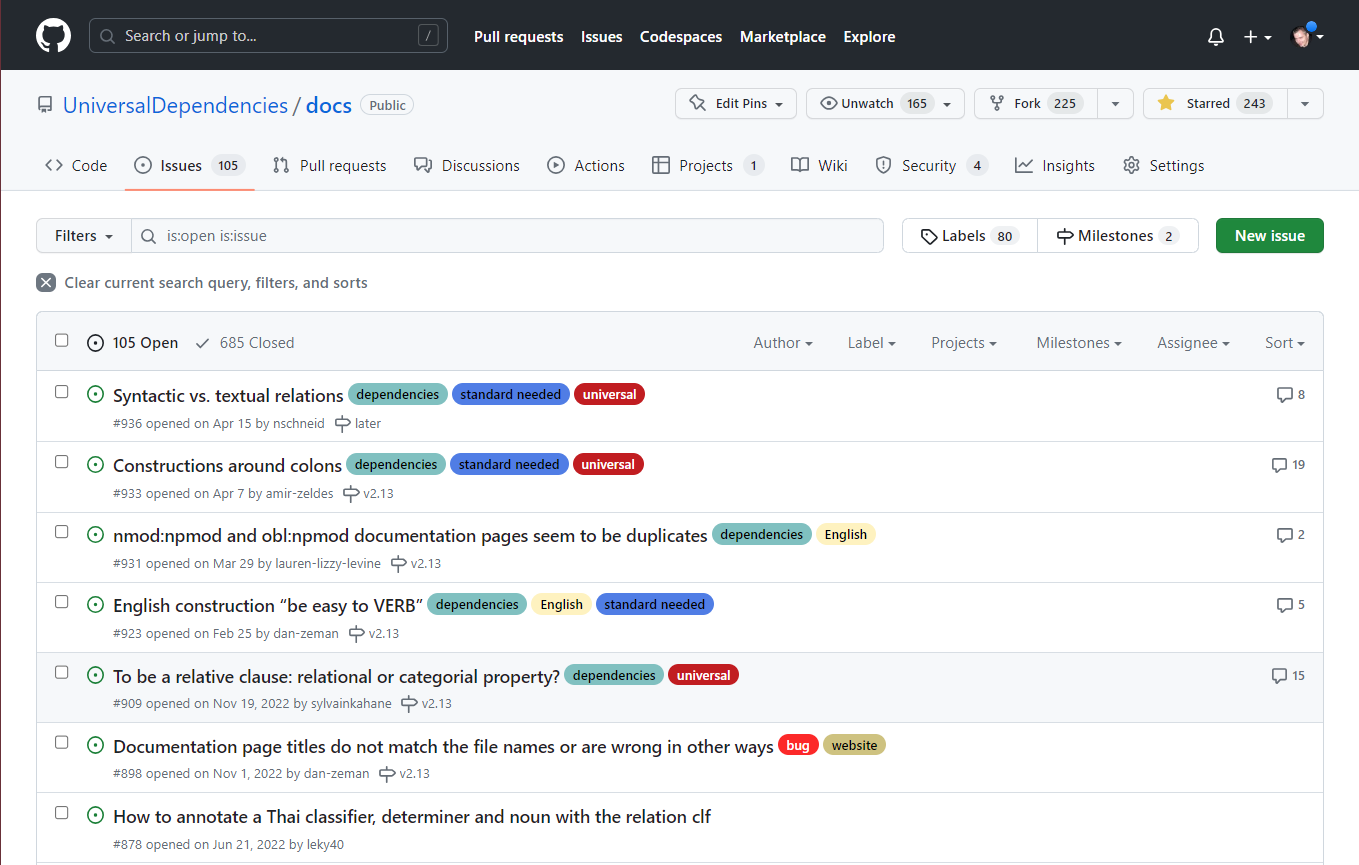
\includegraphics[width=0.9\textwidth]{images/github-issues.png}
  \end{center}
\end{frame}


\begin{frame}{Linguistic Discussion}
  \begin{itemize}
    \item The issue tracker for the \emph{docs} repository is where all the
        UD activity is happening
      \begin{itemize}
        \item Universal guidelines $\Rightarrow$ \emph{docs} issues
        \item Language-specific guidelines $\Rightarrow$ \alert{still
            \emph{docs} issues} (and not treebank repository issues)
          \begin{itemize}
            \item Even if the language has only one treebank
          \end{itemize}
        \item Bugs in a treebank $\Rightarrow$ treebank repository issues
      \end{itemize}
  \end{itemize}
\end{frame}


\begin{frame}
  \frametitle{Where To Get The Data?}
  \textbf{Free text:}
  \begin{itemize}
    \item Plenty of options:
    \begin{itemize}
      \item WikiMedia projects: Wikipedia, Wikinews, \ldots
      \item Public domain texts (varies by country)
      \begin{itemize}
        \item Out of copyright (e.g. old literature, folktales)
        \item Laws/state administrative texts
      \end{itemize}
      \item \alert{Cairo Cicling Corpus}
          \url{https://github.com/UniversalDependencies/cairo/blob/master/translations.txt}
    \end{itemize}
  \end{itemize}
  \textbf{Borderline:}
  \begin{itemize}
    \item Examples from linguistic literature
    \item Shuffled sentences from the web
  \end{itemize}
  \textbf{Non-free text:}
  \begin{itemize}
    \item Contact copyright holders early on
  \end{itemize}
\end{frame}


\begin{frame}[fragile]
  \frametitle{How Much Data?}
  \begin{itemize}
    \item \alert{Required minimum:} 20 sentences and 100 words
    \begin{itemize}
      \item Useful sample: 100 sentences
      \item Very good: 100K tokens
      \item Biggest treebank: 3M tokens
    \end{itemize}
    \item CoNLL-2006, smallest treebank: 29K tokens
    \bigskip
    \item You can add more data for the next release!
  \end{itemize}
\end{frame}


\begin{frame}
  \frametitle{How Long Will It Take?}
  \begin{itemize}
    \item Some approximate numbers:
  \end{itemize}
  \begin{center}
  \begin{tabular}{lrrr}
    \textbf{Language} & \textbf{Annotators} & \textbf{Tokens} & \textbf{Months} \\
    \hline
    Kazakh & 2 & 4,500 & 1 \\
    Buryat & 1 & 10,000 & 3 \\
    Irish &  1 & 23,600 & 12 \\
    \hline
  \end{tabular}
  \end{center}
  In all the above cases, annotation guidelines were developed from scratch
  by people with no prior exposure to UD.
\end{frame}


\begin{frame}{Annotation Tools}
  \begin{itemize}
    \item No official annotation tool
    \item A list of tools:
        \url{http://universaldependencies.org/tools.html}
  \end{itemize}
\end{frame}


\begin{frame}{Bootstrapping}
  \begin{itemize}
    \item<1-> Annotate 20 sentences
    \item<2-> Train a parser on that
    \item<3-> Use it to parse next 100 sentences
    \item<4-> Manually fix annotation
      \begin{itemize}
        \item \alert{UD Requirement: At least UPOS, HEAD and DEPREL must
            be manually verified}
        \item Lemmas and features can be released even if predicted
            automatically (without manual verification of each word)
      \end{itemize}
    \item<5-> Retrain the parser on 120 sentences
    \item<5-> \dots{}
    \bigskip
    \item \url{https://lindat.mff.cuni.cz/services/udpipe/}
    \item \url{https://stanfordnlp.github.io/stanza/}
    \item \url{https://trankit.readthedocs.io/en/latest/overview.html}
  \end{itemize}
\end{frame}


\begin{frame}{Transliteration}
  \url{https://github.com/dan-zeman/translit/blob/main/conllu_translit.pl}

  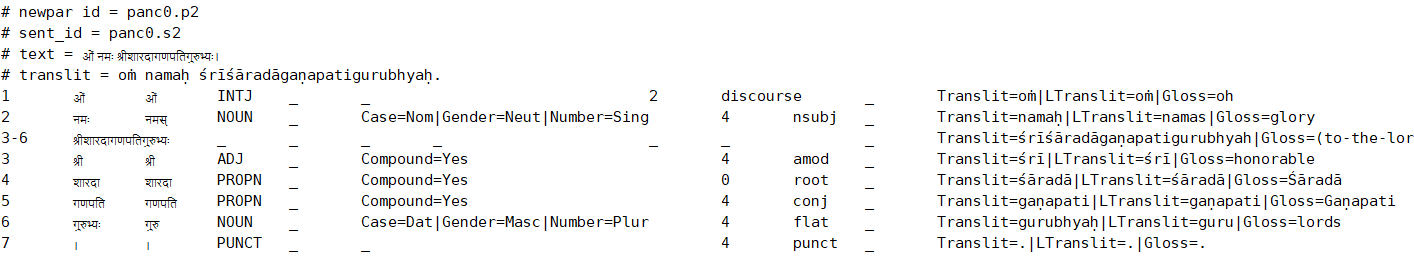
\includegraphics[width=0.95\textwidth]{images/translit-conllu.png}

  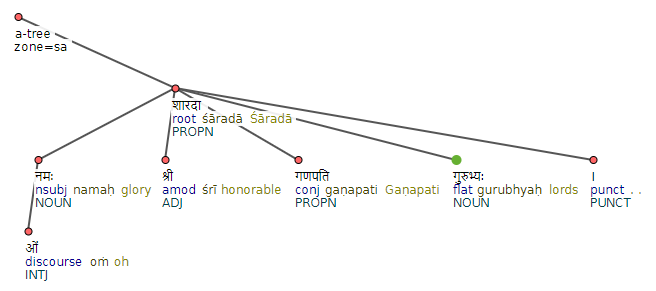
\includegraphics[width=0.95\textwidth]{images/translit-pmltq.png}
\end{frame}


\begin{frame}{Udapi}
  \begin{itemize}
    \item A library and command line tool for processing UD data
      \begin{itemize}
        \item {\bf Python}, Java, Perl
      \end{itemize}
    \item Format conversions
    \item Fixes of systematic errors
    \item Validation tests
    \item Evaluation, filtering, statistics
    \item Tree visualization
    \item \url{https://udapi.github.io}
      \begin{itemize}
        \item
            \url{https://ufal.mff.cuni.cz/~zeman/vyuka/deptreebanks/NPFL075-working-with-UD.pdf}
      \end{itemize}
  \end{itemize}
\end{frame}


{\nologo\begin{frame}{Tree Visualization Tools}
  {\tt cat en\_ewt-ud-dev.conllu | udapy -T | less -R}
  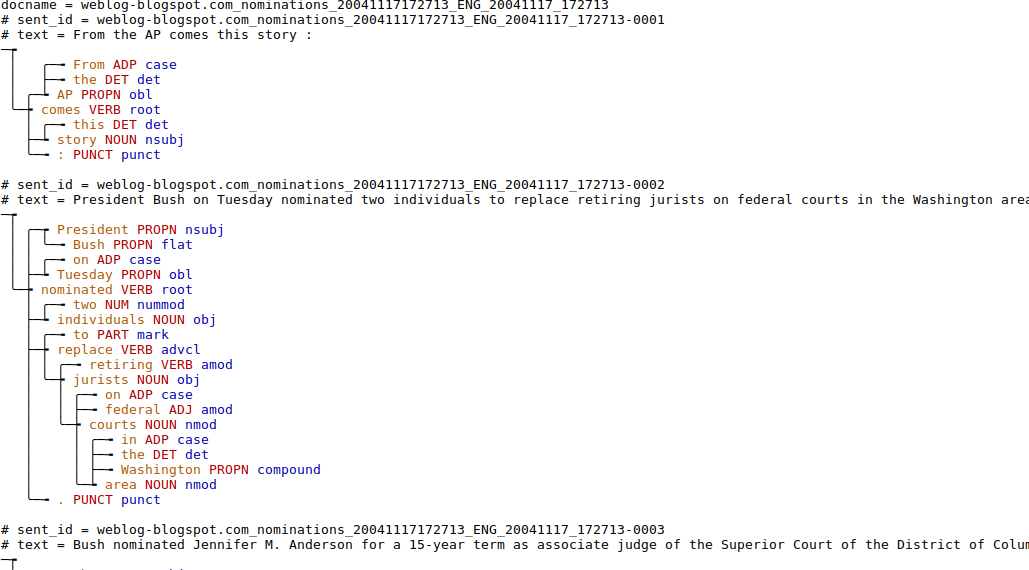
\includegraphics[width=\linewidth,height=\textheight,keepaspectratio]{images/udapi_viz.png}
\end{frame}}


\begin{frame}{Tree Visualization Tools}
  {\tt cat en\_ewt-ud-dev.conllu | udapy write.Tikz}

  \scalebox{0.9}{
  \begin{dependency}
    \begin{deptext}
      % sent_id = reviews-140302-0004
      % text = Also, they have great customer service and a very knowledgeable staff
      Also \& ,     \& they \& have \& great \& customer \& service \& and   \& a   \& very \& knowledgeable \& staff \\
      ADV  \& PUNCT \& PRON \& VERB \& ADJ   \& NOUN     \& NOUN    \& CCONJ \& DET \& ADV  \& ADJ           \& NOUN  \\
    \end{deptext}
    \depedge{4}{1}{advmod} \depedge{4}{2}{punct} \depedge{4}{3}{nsubj}
    \deproot{4}{root} \depedge{7}{5}{amod} \depedge{7}{6}{compound}
    \depedge{4}{7}{obj} \depedge{12}{8}{cc} \depedge{12}{9}{det}
    \depedge{11}{10}{advmod} \depedge{12}{11}{amod} \depedge{7}{12}{conj}
  \end{dependency}
  }
\end{frame}


\begin{comment}
{\nologo\begin{frame}{Tree Visualization Tools}
  {\tt http://spyysalo.github.io/conllu.js/}

  {\tt http://spyysalo.github.io/annodoc/sdparse.html}

  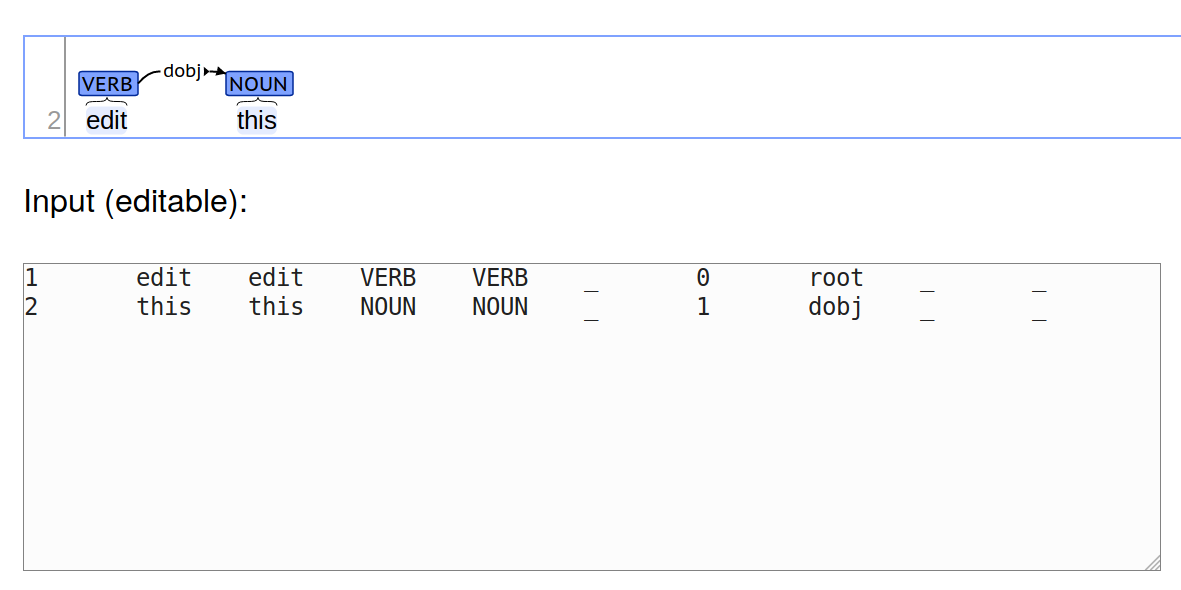
\includegraphics[width=\linewidth,height=\textheight,keepaspectratio]{images/onlinebrat.png}
\end{frame}}
\end{comment}


\begin{frame}
  \frametitle{Summary}
  \textbf{What you need to do}
  \begin{itemize}
    \item Join the project
    \item Start annotating or converting
    \item Ask if you get stuck!
  \end{itemize}
\end{frame}


\end{document}
